% LUMA: Lightweight Attention-UNet for Real-Time Low-Light Image Enhancement
% Build: see report/README.md (Overleaf, or `latexmk -pdf main.tex`).
% EVERY number about our results comes from report/generated/*.tex, which
% src/collect_results.py writes from the JSON files in results/. Do not type numbers here.
\documentclass[10pt,twocolumn,letterpaper]{article}
\usepackage[margin=0.8in]{geometry}
\usepackage{times}
\usepackage{amsmath,amssymb}
\usepackage{graphicx}
\usepackage{booktabs}
\usepackage{xcolor}
\usepackage{tikz}
\usetikzlibrary{positioning,arrows.meta,fit}
\usepackage[hidelinks]{hyperref}
\usepackage[numbers,sort&compress]{natbib}
\usepackage{caption}
\captionsetup{font=small}

\newcommand{\pending}{\textcolor{red}{[pending]}}
\newcommand{\todo}[1]{\textcolor{red}{[TODO: #1]}}
\IfFileExists{generated/numbers.tex}{% AUTO-GENERATED by src/collect_results.py from results/. Do not edit.
\providecommand{\pending}{\textcolor{red}{[pending]}}
\newcommand{\OursParamsK}{\pending{}}
\newcommand{\OursParamsM}{\pending{}}
\newcommand{\OursMACs}{\pending{}}
\newcommand{\OursMACsFHD}{\pending{}}
\newcommand{\OursFPS}{\pending{}}
\newcommand{\OursFPSHalf}{\pending{}}
\newcommand{\OursFPSFHD}{\pending{}}
\newcommand{\OursFPSFHDHalf}{\pending{}}
\newcommand{\GPUName}{\pending{}}
\newcommand{\OursPSNRLolVOne}{\pending{}}
\newcommand{\OursPSNRLolVOneGTMean}{\pending{}}
\newcommand{\OursSSIMLolVOne}{\pending{}}
\newcommand{\OursSSIMLolVOneGTMean}{\pending{}}
\newcommand{\OursLPIPSLolVOne}{\pending{}}
\newcommand{\OursLPIPSLolVOneGTMean}{\pending{}}
\newcommand{\OursPSNRLolVTwoReal}{\pending{}}
\newcommand{\OursPSNRLolVTwoRealGTMean}{\pending{}}
\newcommand{\OursSSIMLolVTwoReal}{\pending{}}
\newcommand{\OursSSIMLolVTwoRealGTMean}{\pending{}}
\newcommand{\OursLPIPSLolVTwoReal}{\pending{}}
\newcommand{\OursLPIPSLolVTwoRealGTMean}{\pending{}}
\newcommand{\OursPSNRLolVTwoSyn}{\pending{}}
\newcommand{\OursPSNRLolVTwoSynGTMean}{\pending{}}
\newcommand{\OursSSIMLolVTwoSyn}{\pending{}}
\newcommand{\OursSSIMLolVTwoSynGTMean}{\pending{}}
\newcommand{\OursLPIPSLolVTwoSyn}{\pending{}}
\newcommand{\OursLPIPSLolVTwoSynGTMean}{\pending{}}
\newcommand{\ZeroDCEPSNRLolVOne}{\pending{}}
\newcommand{\ZeroDCEPPPSNRLolVOne}{\pending{}}
\newcommand{\RetinexNetPSNRLolVOne}{\pending{}}
\newcommand{\EnlightenGANPSNRLolVOne}{\pending{}}
\newcommand{\RetinexformerPSNRLolVOne}{\pending{}}
\newcommand{\OursNIQEDICM}{\pending{}}
\newcommand{\OursNIQELIME}{\pending{}}
\newcommand{\OursNIQEMEF}{\pending{}}
\newcommand{\OursNIQENPE}{\pending{}}
\newcommand{\OursNIQEVV}{\pending{}}
}{}
% Safe fallbacks if collect_results.py has not been run yet.
\providecommand{\OursParamsK}{\pending}\providecommand{\OursParamsM}{\pending}
\providecommand{\OursMACs}{\pending}\providecommand{\OursMACsFHD}{\pending}
\providecommand{\OursFPS}{\pending}\providecommand{\OursFPSHalf}{\pending}
\providecommand{\OursFPSFHD}{\pending}\providecommand{\OursFPSFHDHalf}{\pending}
\providecommand{\GPUName}{\pending}
\providecommand{\OursPSNRLolVOne}{\pending}\providecommand{\OursSSIMLolVOne}{\pending}
\providecommand{\OursLPIPSLolVOne}{\pending}
\providecommand{\OursPSNRLolVTwoReal}{\pending}\providecommand{\OursPSNRLolVTwoSyn}{\pending}
\providecommand{\OursPSNRLolVOneGTMean}{\pending}
\providecommand{\RetinexformerPSNRLolVOne}{\pending}

% Include a generated table if it exists, otherwise a visible placeholder.
\newcommand{\gentable}[1]{\IfFileExists{generated/#1.tex}{\input{generated/#1.tex}}{%
  \begin{table}[t]\centering\fbox{\parbox{0.9\columnwidth}{\centering\small
  \pending{} table \texttt{\detokenize{#1}} (run \texttt{src/collect\_results.py})}}\end{table}}}
\newcommand{\genfigure}[3]{\IfFileExists{#1}{%
  \begin{figure}[t]\centering\includegraphics[width=#2]{#1}\caption{#3}\end{figure}}{%
  \begin{figure}[t]\centering\fbox{\parbox{0.9\columnwidth}{\centering\small\pending{} figure
  \texttt{\detokenize{#1}}}}\caption{#3}\end{figure}}}

\title{\textbf{LUMA: A Lightweight Attention-UNet for\\Real-Time Low-Light Image Enhancement}}
\author{Asad\\\small\url{https://github.com/Asad3404/LUMA}}
\date{}

\begin{document}
\maketitle

% ---------------------------------------------------------------------------
\begin{abstract}
Photographs taken in low light are dark, noisy and colour-shifted, and many
downstream vision systems must handle them in real time on modest hardware.
We present LUMA, a compact U-shaped convolutional network that combines
depthwise-separable convolutions, CBAM-style channel and spatial attention,
and additive attention gates on the skip connections, and predicts a
residual added to the input. The model has \OursParamsK{}K parameters and
requires \OursMACs{} GMACs for a $600\times400$ image. Trained with a
combination of Charbonnier, SSIM, VGG perceptual and colour losses, it reaches
\OursPSNRLolVOne{}~dB PSNR and \OursSSIMLolVOne{} SSIM on the LOL-v1 test
set \emph{without} ground-truth mean correction, and runs at
\OursFPS{}~FPS (FP32) / \OursFPSHalf{}~FPS (FP16) at $600\times400$ on a
\GPUName{}. All baselines are re-evaluated with identical metric code, and
ablations isolate the contribution of each attention component, each loss
term and the network width. Code, configurations, logs and every reported
number are released.
\end{abstract}

% ---------------------------------------------------------------------------
\section{Introduction}
Low-light enhancement aims to recover a well-exposed, natural-looking image
from a photograph captured under insufficient illumination. Beyond
photography, it is a pre-processing step for night-time driving, surveillance
and robotics, where latency and compute budgets are tight. Recent
transformer-based methods such as Retinexformer~\cite{cai2023retinexformer}
reach high fidelity on the LOL benchmarks~\cite{wei2018deep,yang2021sparse},
but even they use more than a million parameters and tens of GFLOPs per
image. At the other extreme, curve-estimation networks such as
Zero-DCE~\cite{guo2020zero,li2021learning} are tiny and fast but, being
trained without paired supervision, are less faithful to the reference images.

This project investigates the middle ground: \emph{how much fidelity can a
sub-million-parameter, real-time convolutional network achieve when attention
is spent carefully?} Our contributions are:
\begin{itemize}\itemsep0pt
\item A configurable lightweight Attention-UNet (\S\ref{sec:method}) in which
  every component (convolution type, channel/spatial attention, attention
  gates, upsampling, global residual) can be switched off from a config file.
\item An honest evaluation protocol (\S\ref{sec:protocol}): PSNR/SSIM
  \emph{without} GT-mean correction as the main metric, the same metric code
  for all baselines, and fixed seeds with every config saved.
\item Efficiency measurements with proper GPU synchronisation, ONNX export and
  FP16 inference (\S\ref{sec:efficiency}), and ablations of attention, loss
  and width (\S\ref{sec:ablations}).
\end{itemize}

% ---------------------------------------------------------------------------
\section{Related Work}
\paragraph{Retinex-based methods.} Retinex theory~\cite{land1977retinex}
models an image as the product of reflectance and illumination.
RetinexNet~\cite{wei2018deep} learns this decomposition with paired LOL data,
KinD~\cite{zhang2019kind} adds dedicated restoration branches, and
Retinexformer~\cite{cai2023retinexformer} uses illumination-guided
self-attention in a one-stage transformer.

\paragraph{Curve estimation and unpaired learning.} Zero-DCE~\cite{guo2020zero}
predicts pixel-wise quadratic curves with a seven-layer CNN trained by
non-reference losses, and Zero-DCE++~\cite{li2021learning} reduces it further
with depthwise-separable convolutions. EnlightenGAN~\cite{jiang2021enlightengan}
trains an attention-guided U-Net adversarially on unpaired data.

\paragraph{Attention in CNNs.} Squeeze-and-Excitation~\cite{hu2018squeeze}
and ECA~\cite{wang2020eca} re-weight channels from globally pooled
statistics; CBAM~\cite{woo2018cbam} adds a spatial attention map; Attention
U-Net~\cite{oktay2018attention} gates encoder skip features with decoder
signals. Depthwise-separable convolutions~\cite{howard2017mobilenets} are the
standard tool for cutting the cost of convolutions. We combine these
inexpensive mechanisms in a single small model.

% ---------------------------------------------------------------------------
\section{Method}\label{sec:method}
\begin{figure*}[t]
\centering
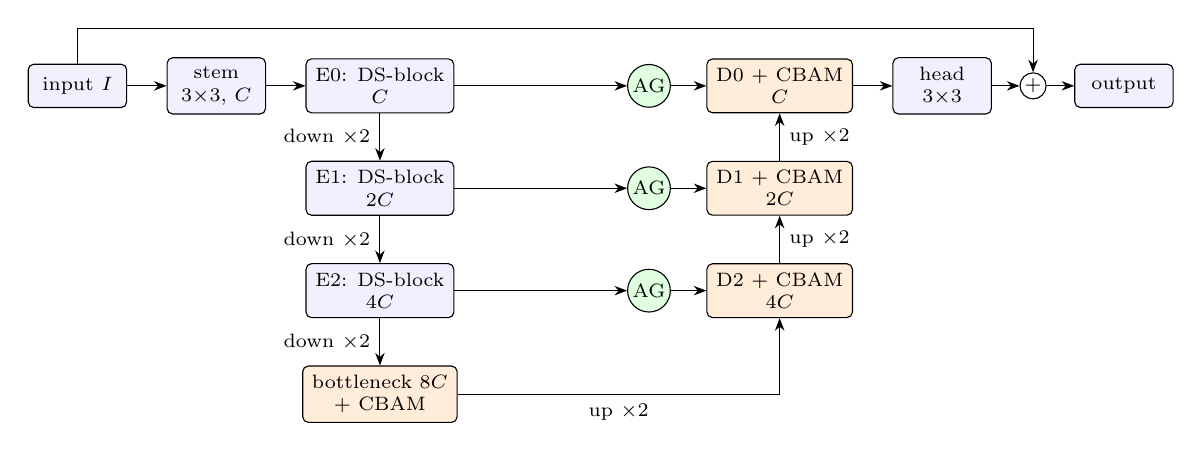
\begin{tikzpicture}[font=\scriptsize, node distance=0.35cm and 0.5cm,
  blk/.style={draw, rounded corners=2pt, minimum height=0.55cm, minimum width=1.25cm, align=center, fill=blue!6},
  att/.style={draw, rounded corners=2pt, minimum height=0.55cm, minimum width=1.25cm, align=center, fill=orange!15},
  gate/.style={draw, circle, inner sep=1pt, fill=green!12},
  arr/.style={-{Stealth[length=1.6mm]}}]
\node[blk] (in) {input $I$};
\node[blk, right=of in] (stem) {stem\\3$\times$3, $C$};
\node[blk, right=of stem] (e0) {E0: DS-block\\$C$};
\node[blk, below=0.6cm of e0] (e1) {E1: DS-block\\$2C$};
\node[blk, below=0.6cm of e1] (e2) {E2: DS-block\\$4C$};
\node[att, below=0.6cm of e2] (bn) {bottleneck $8C$\\+ CBAM};
\node[att, right=3.2cm of e2] (d2) {D2 + CBAM\\$4C$};
\node[att, right=3.2cm of e1] (d1) {D1 + CBAM\\$2C$};
\node[att, right=3.2cm of e0] (d0) {D0 + CBAM\\$C$};
\node[gate, left=0.45cm of d2] (g2) {AG};
\node[gate, left=0.45cm of d1] (g1) {AG};
\node[gate, left=0.45cm of d0] (g0) {AG};
\node[blk, right=of d0] (head) {head\\3$\times$3};
\node[circle, draw, right=0.35cm of head, inner sep=0.5pt] (plus) {$+$};
\node[blk, right=0.35cm of plus] (out) {output};
\draw[arr] (in) -- (stem); \draw[arr] (stem) -- (e0);
\draw[arr] (e0) -- node[left]{down $\times$2} (e1);
\draw[arr] (e1) -- node[left]{down $\times$2} (e2);
\draw[arr] (e2) -- node[left]{down $\times$2} (bn);
\draw[arr] (bn) -| node[pos=0.25, below]{up $\times$2} (d2);
\draw[arr] (d2) -- node[right]{up $\times$2} (d1);
\draw[arr] (d1) -- node[right]{up $\times$2} (d0);
\draw[arr] (e2) -- (g2); \draw[arr] (g2) -- (d2);
\draw[arr] (e1) -- (g1); \draw[arr] (g1) -- (d1);
\draw[arr] (e0) -- (g0); \draw[arr] (g0) -- (d0);
\draw[arr] (d0) -- (head); \draw[arr] (head) -- (plus); \draw[arr] (plus) -- (out);
\draw[arr] (in.north) -- ++(0,0.45) -| (plus.north);
\end{tikzpicture}
\caption{LUMA architecture (4 levels, $C{=}16$). DS-block: two depthwise-separable
convolutions with LeakyReLU and a residual shortcut. AG: additive attention gate
driven by the upsampled decoder feature. CBAM: channel then spatial attention.
Downsampling uses learned $2\times2$ stride-2 convolutions, upsampling is
bilinear followed by a $1\times1$ projection. The prediction is added to the input
(global residual) and clamped to $[0,1]$ at inference.}
\label{fig:arch}
\end{figure*}

\paragraph{Overview.} Fig.~\ref{fig:arch} shows the network. A $3\times3$ stem
maps the RGB input to $C$ channels. The encoder has three levels of
DS-blocks with $C$, $2C$ and $4C$ channels, separated by learned
$2\times2$ stride-2 convolutions; the bottleneck works at $8C$ channels and
$1/8$ resolution. Each decoder level upsamples, gates the corresponding
encoder feature, concatenates, fuses with a $1\times1$ convolution and applies
a DS-block followed by attention. A $3\times3$ head predicts a residual
$R$, and the output is $\hat{Y}=\mathrm{clip}(I+R,0,1)$. Inputs whose sides are
not multiples of 8 are reflect-padded and the output is cropped back.

\paragraph{DS-block.} A depthwise $3\times3$ convolution followed by a
pointwise $1\times1$ convolution~\cite{howard2017mobilenets} costs roughly
$1/9$ of a standard $3\times3$ convolution when the channel count is large. Each block applies
two of them with LeakyReLU, plus an identity (or $1\times1$) shortcut.

\paragraph{Channel and spatial attention.} Low-light degradation is not
uniform: noise and colour casts depend on the channel, and under-exposure is
spatially varying. We use CBAM~\cite{woo2018cbam}: channel weights
$\sigma(\mathrm{MLP}(\mathrm{AvgPool}(F))+\mathrm{MLP}(\mathrm{MaxPool}(F)))$
followed by a spatial map $\sigma(f^{7\times7}([\mathrm{mean}_c F;\max_c F]))$.
ECA~\cite{wang2020eca} and SE~\cite{hu2018squeeze} are available as drop-in
channel modules.

\paragraph{Attention gates.} Following Attention U-Net~\cite{oktay2018attention},
each skip feature $x$ is multiplied by
$\alpha=\sigma(\psi(\mathrm{ReLU}(W_g g + W_x x)))$, where $g$ is the upsampled
decoder feature. Encoder features of dark images carry a lot of
noise, and the gate lets the decoder decide where to rely on them.

\paragraph{Losses.} With prediction $\hat{Y}$ and reference $Y$,
\begin{equation}
\mathcal{L}=\lambda_1\mathcal{L}_{\mathrm{Charb}}+\lambda_2(1-\mathrm{SSIM})
+\lambda_3\mathcal{L}_{\mathrm{VGG}}+\lambda_4\mathcal{L}_{\mathrm{col}},
\end{equation}
where $\mathcal{L}_{\mathrm{Charb}}=\mathrm{mean}\sqrt{(\hat Y-Y)^2+\epsilon^2}$
($\epsilon{=}10^{-3}$)~\cite{charbonnier1994two}, SSIM~\cite{wang2004image} uses an
$11\times11$ Gaussian window, $\mathcal{L}_{\mathrm{VGG}}$ is the $L_1$ distance of
VGG-19~\cite{simonyan2015very} features at relu1\_2, relu2\_2, relu3\_4 and
relu4\_4~\cite{johnson2016perceptual}, and $\mathcal{L}_{\mathrm{col}}$ is the mean
$1-\cos$ angle between predicted and reference RGB vectors. We use
$(\lambda_1,\lambda_2,\lambda_3,\lambda_4)=(1,0.3,0.05,0.1)$ (\texttt{configs/base.yaml});
these were set once and not tuned on the test set.

% ---------------------------------------------------------------------------
\section{Experimental Setup}\label{sec:protocol}
\paragraph{Data.} We train on the 485 LOL-v1~\cite{wei2018deep} training pairs
and test on its 15 test pairs ($600\times400$). We also report LOL-v2-Real
(689/100 pairs) and LOL-v2-Synthetic (900/100 pairs)~\cite{yang2021sparse},
and no-reference NIQE~\cite{mittal2013making} on DICM~\cite{lee2013contrast},
LIME~\cite{guo2017lime}, MEF~\cite{ma2015perceptual}, NPE~\cite{wang2013naturalness}
and VV. Our download script verifies the pair counts and also measures how many
LOL-v1 images reappear in LOL-v2-Real (\texttt{results/data/data\_summary.json}),
because the two datasets share captures.

\paragraph{Training.} Random $256\times256$ crops with flips and $90^\circ$
rotations, batch size 8, AdamW~\cite{loshchilov2019decoupled} (lr $2\times10^{-4}$,
weight decay $10^{-4}$), 3 warm-up epochs then cosine
annealing~\cite{loshchilov2017sgdr} to $10^{-6}$, gradient clipping at 1.0,
and mixed precision~\cite{micikevicius2018mixed}. The main model is trained for
300 epochs of 485 iterations; ablations use a shared 100-epoch schedule.
Validation runs every 5 epochs on the LOL-v1 test split and the checkpoint with
the best validation PSNR is kept. Because the LOL-v1 test split is also used for
model selection (standard practice for this benchmark, which has no separate
validation split), our numbers are slightly optimistic; we report the epoch
selected in \texttt{results/}. Seed 42 everywhere; every run stores its exact
configuration next to its checkpoint.

\paragraph{Metrics.} PSNR is computed on float images in $[0,1]$ after clamping;
SSIM is the MATLAB-style formulation~\cite{wang2004image} computed per RGB
channel on 8-bit images and averaged; LPIPS uses AlexNet~\cite{zhang2018unreasonable}.
These mirror the Retinexformer evaluation code. \textbf{No GT-mean correction}
is applied to the main results. Several works~\cite{zhang2019kind,wang2022low}
rescale the output to the mean brightness of the ground truth, which uses
test-time ground truth. We list such scores only in a separate, labelled
supplementary table.

\paragraph{Baselines.} Zero-DCE and Zero-DCE++ (official weights; both
architectures re-implemented with identical layer names so the official
weights load strictly), EnlightenGAN (official weights converted to ONNX),
RetinexNet (unofficial PyTorch port and its checkpoint, since the official
release is TensorFlow~1), and Retinexformer (official code and per-dataset
weights). All are run on the same images with the same metric code. Any
baseline that cannot be run falls back to published numbers marked
``reported\textsuperscript{\dag}''.

% ---------------------------------------------------------------------------
\section{Results}
\gentable{main_results}
\gentable{comparison_lol_v1}

\paragraph{Fidelity.} Table~\ref{tab:main_results} lists our model on each
paired test set and Table~\ref{tab:comparison_lol_v1} compares it with the
baselines on LOL-v1. Our model obtains \OursPSNRLolVOne{}~dB / \OursSSIMLolVOne{}
SSIM / \OursLPIPSLolVOne{} LPIPS on LOL-v1, compared with
\RetinexformerPSNRLolVOne{}~dB for Retinexformer measured with the same code.
\todo{Interpret the comparison once the numbers are in: where LUMA sits between
the curve-based methods and Retinexformer, and how large the PSNR/compute
trade-off is.}

\genfigure{../results/figures/psnr_vs_macs.png}{\columnwidth}{PSNR on LOL-v1
versus compute (GMACs per $600\times400$ image, log scale).}

\paragraph{Qualitative results.} Fig.~\ref{fig:qual} shows inputs, baseline
outputs, ours and the ground truth with zoomed crops.
\todo{Describe what is visible: noise in dark regions, colour fidelity,
over/under-exposure.}

\genfigure{../results/figures/lol_v1_1.png}{\textwidth}{Qualitative comparison
on LOL-v1. Red boxes are enlarged in the bottom row.\label{fig:qual}}

\gentable{niqe}
\paragraph{Generalisation.} On sets without ground truth we report NIQE
(lower is better) in Table~\ref{tab:niqe}. NIQE is only a weak proxy for
perceived quality and should be read together with the qualitative results.
\todo{Comment on the NIQE results.}

\gentable{main_results_gtmean}
\paragraph{GT-mean-corrected scores (supplementary).} For comparison with
papers that use it, Table~\ref{tab:main_results_gtmean} gives scores after
rescaling our output to the reference mean brightness
(\OursPSNRLolVOneGTMean{}~dB on LOL-v1). These scores use the ground truth at test
time and are not our main result.

% ---------------------------------------------------------------------------
\section{Efficiency}\label{sec:efficiency}
\gentable{efficiency}
Table~\ref{tab:efficiency} reports latency and throughput at batch size 1
after 50 warm-up runs, averaged over 200 timed runs with
\texttt{torch.cuda.synchronize()} around each run. Image decoding and
host--device copies are excluded. At $600\times400$ the model reaches
\OursFPS{}~FPS in FP32 and \OursFPSHalf{}~FPS in FP16. At $1920\times1080$
(\OursMACsFHD{} GMACs) it reaches \OursFPSFHD{} / \OursFPSFHDHalf{}~FPS.
The ONNX export is checked against PyTorch: the maximum absolute output difference
is stored in \texttt{results/benchmark/*\_onnx.json}. Note that MAC counts from
\texttt{thop} cover convolutions and linear layers; element-wise operations
(sigmoids, multiplications in attention) are not included.

% ---------------------------------------------------------------------------
\section{Ablation Studies}\label{sec:ablations}
All variants are trained with the same 100-epoch schedule and seed and are
evaluated on LOL-v1. The reference row (CBAM + gates, full loss, $C{=}16$) is
shared between the three tables.

\gentable{ablation_attention}
\gentable{ablation_loss}
\gentable{ablation_width}

\paragraph{Attention.} Table~\ref{tab:ablation_attention}.
\todo{Which component contributes most? Is the gain worth the FPS cost?}

\paragraph{Loss terms.} Table~\ref{tab:ablation_loss}.
\todo{Effect of SSIM / perceptual / colour terms on PSNR vs LPIPS.}

\paragraph{Width.} Table~\ref{tab:ablation_width}.
\todo{Quality-vs-speed trade-off across widths 8/16/32.}

% ---------------------------------------------------------------------------
\section{Limitations}
\begin{itemize}\itemsep0pt
\item LOL-v1 has only 15 test images, so differences of a few tenths of a dB
  are within run-to-run variation. We train each configuration once (single
  seed); multiple seeds would be needed to give confidence intervals.
\item Model selection uses the LOL-v1 test split (no separate validation set),
  as is common on this benchmark, which slightly favours the reported numbers.
\item LOL-v1 and LOL-v2-Real share images, so cross-dataset numbers between
  them are not independent (overlap counts in \texttt{results/data/}).
\item Baselines are run with released weights trained on different data and
  protocols. RetinexNet uses an unofficial port, and Zero-DCE++ is run at full
  resolution rather than with its default down-scaling.
\item The model processes frames independently, so video output can flicker.
  It does not handle extreme noise (very short exposures) or RAW input.
\end{itemize}

% ---------------------------------------------------------------------------
\section{Conclusion}
We built and evaluated LUMA, a \OursParamsK{}K-parameter Attention-UNet for
low-light enhancement that reaches \OursPSNRLolVOne{}~dB on LOL-v1 without
GT-mean correction while running at \OursFPS{}~FPS at $600\times400$ on a
\GPUName{}. Every number in this report is produced by scripts in the
repository and can be reproduced on a free Colab GPU. Future work includes
temporal consistency for video, joint denoising, INT8 quantisation, and
measuring the effect on downstream detection in the dark (e.g.\ ExDark).

\small
\bibliographystyle{unsrtnat}
\bibliography{references}
\end{document}
